 
\subsection{Mechanisch}
Het wagentje is een vierwieler. Een model van de wagen bevindt zich in Figuur~\ref{image:auto-resultaat}. Aan de voorkant is langs beide kanten een 
rechthoek uitgesneden. Deze uitsnijdingen zorgen ervoor dat de wielen genoeg 
plaats hebben om te kunnen draaien. Achteraan is een as waarop beide 
achterwielen gefixeerd zijn. 
Op de achteras is een elektromotor (MM28) aangesloten die zorgt voor de 
aandrijving van de wagen. De motor staat via een reeks van tandwielen in 
verbinding met de achteras. Deze tandwielen zorgen voor de nodige overbrenging 
naar de wielen. Deze overbrenging heeft een verhouding van 1 op 125, waarbij de 
achteras 125 keer trager draait dan de motor.  De wagen remt door het 
uitschakelen van de motor. De rolweerstand en de wrijving veroorzaakt door de 
overbrenging, is voldoende om de wagen op tijd te laten stoppen.
De voorwielen staan elk op een aparte as. De twee assen zijn verbonden met een 
stuurmechanisme waardoor de voorwielen altijd parallel staan ten opzichte van 
elkaar. De wielen kunnen wel schuin komen te staan ten opzichte van de 
middenlijn. Hierdoor kan de auto gemakkelijk bochten nemen. De assen bewegen 
onder impuls van een servomotor. Deze servomotor drijft het sturingsmechanisme 
aan waardoor de wielen een hoek van ten hoogste 45 graden kunnen maken ten 
opzichte van de middenlijn. De afstandssensor is bovenop het sturingsmechanisme 
aangebracht, helemaal vooraan de wagen.
\begin{figure}
 \centering
 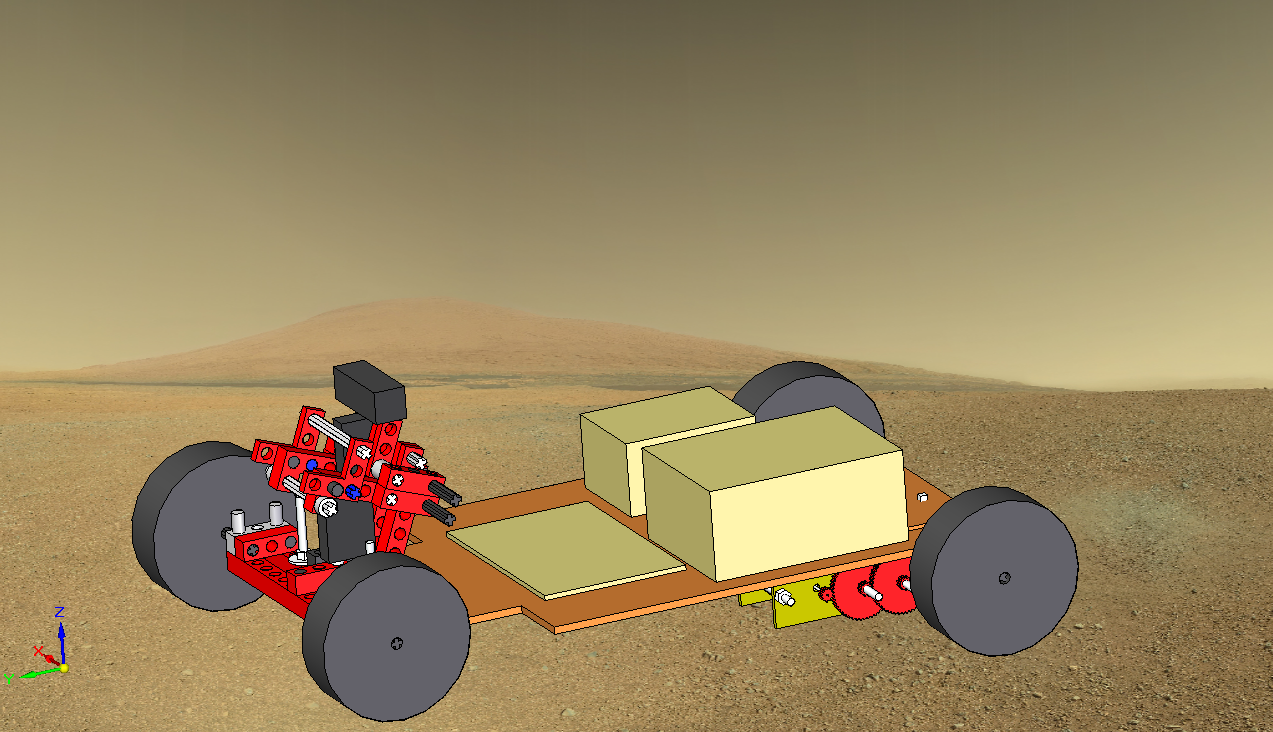
\includegraphics[width=\linewidth]{conceptkeuze-ontwerp/mechanisch/auto-resultaat.png}
 \caption{3D-model van het wagentje gemaakt met Solid Edge.}
 \label{image:auto-resultaat}
\end{figure}

De bodemplaat wordt schuin gemonteerd op beide assen en ligt hoger aan de 
achterkant. De plaat staat schuin omdat de motor en overbrenging aan de 
onderkant gemonteerd zijn. Hierdoor is er genoeg plaats over aan de bovenkant 
voor de elektronica en kunnen de tandwielen de draden niet beschadigen. 
Op de bovenkant van de bodemplaat komt de Arduino, de batterij en het Printed 
Circuit Board (PCB). Het gewicht wordt hierbij zo centraal mogelijk geplaatst, 
zodat het stuurmechanisme nog genoeg grip heeft om de koers van de wagen te 
wijzigen, zonder daarbij te veel weerstand te veroorzaken voor de servomotor. 
Bij een te hoge weerstand zou de servomotor de wielen niet op tijd kunnen 
draaien en zou de wagen de muur raken.

Het voordeel aan dit ontwerp is dat de stabiliteit, snelheid en wendbaarheid 
geoptimaliseerd worden. 
